\documentclass[beleg,zihtitle,american,final,hyperref,utf8,open=any,oneside]{zihpub}

% Libraries
\usepackage{setspace}
\usepackage{booktabs} % for \toprule, \midrule, \bottomrule, \cmidrule
\usepackage{pgfplots}
\usepackage{enumitem}
\usepackage{csquotes}
\pgfplotsset{compat=1.18}
\usepackage{siunitx}
\sisetup{
  per-mode = symbol,
  group-minimum-digits = 4,
  detect-mode,
  detect-weight,
  detect-family
}
\usepgfplotslibrary{groupplots,statistics,fillbetween,dateplot}
\newcommand{\BibLaTeX}{\textsc{Bib}\LaTeX}

\author{Benjamin-Elias Probst}
\title{Deduplication in Data Storage Systems}
\bibfiles{doku}

\birthday{11. April 1996}
\placeofbirth{Potsdam}
\matno{4510512}

\betreuer{Dr. Alexander Krause}
\hsl{Prof. Dr. Wolfgang Lehner}

\begin{document}


\let\cleardoublepage\clearpage
\selectlanguage{american} % ensure US English is active

% ---------------------------------------------------------
% ZOPP structure (headings only; content to be added later)
% ---------------------------------------------------------

% (Optional) Abstract
\chapter*{Abstract}
% Brief, 5–8 sentences: problem, objective, approach, key results, impact.
% \addcontentsline{toc}{chapter}{Abstract} % uncomment if you want it in the ToC
Deduplication is a technique in modern storage systems for identifying redundant data and storing it only once, thereby saving storage space and bandwidth. This paper outlines the motivation and concept of deduplication and distinguishes it from related approaches such as compression. We trace the historical development of deduplication from early file systems (LBFS, Venti) to enterprise backup solutions (Data Domain’s DDFS) and latency-sensitive primary storage methods (iDedup). We present a taxonomy of deduplication methods along key dimensions: detection principle, granularity, timing (inline vs. post-process), architecture (source vs. target), and primary vs. secondary storage. The application of deduplication is examined in various data storage systems including relational databases, object stores, time series databases, and scalable platforms like Kafka and Hadoop. An initial evaluation highlights that deduplication provides significant benefits in backup and archival systems, must be carefully balanced for performance in primary storage and databases, and faces challenges in distributed and big data environments. Finally, based on these insights, we derive research objectives aimed at developing adaptive, scalable deduplication strategies for future storage systems.

% -----------------------------------------------
% Main Content
% -----------------------------------------------

\chapter{Introduction and Motivation}
\label{ch:einleitung}
In modern IT systems, enormous volumes of data are generated that often contain redundant content. \emph{Data deduplication} (also called deduplication) refers to techniques for detecting such redundant data and storing them only once. In this way, storage requirements and transmission costs can be drastically reduced. Deduplication is used particularly in data backup environments (backups) to save storage space and network bandwidth, since e.g. identical email attachments or files that are backed up multiple times need only be stored once. Deduplication also plays an important role in cloud storage and modern data storage systems, as identical data that are stored multiple times by different users or applications only need to be kept once. Through this increase in efficiency, companies can reduce costs for storage media, power, and cooling while simultaneously accelerating data transfer.

Throughout this report, the focus is on \textbf{physical deduplication}: whether redundant payload bytes result in shared or eliminated \emph{on-disk} representations, and how such effects become visible across storage layers. This is distinct from \textbf{compression}, which reduces the footprint of each object instance without cross-object sharing. Beyond intentionally engineered deduplication, this work also treats \textbf{deduplication as an emergent effect} that can arise unintentionally from database semantics and maintenance (e.g., upserts, merge policies, compaction, or TTL/GC).

\paragraph{Module context and deliverable.}
The work is written in the context of the TU Dresden module \emph{Analyse eines Forschungsthemas} (Diplom-Informatik, Prüfungsordnung $\geq$2010) and therefore combines a structured literature analysis with an empirical exploration on a real system. \cite{TUDresdenModuleINF-D-960}

\paragraph{Research questions.}
\begin{enumerate}[label=RQ\arabic*:, leftmargin=*, itemsep=0.2em]
  \item What is \emph{physical} deduplication in database systems, and how does it differ from compression and purely logical duplicate prevention?
  \item Which storage-architecture mechanisms in common systems can be interpreted as deduplication (full/partial) or lead to deduplication-like effects (indirect)?
  \item How do duplicate ratios (0--99\%), placement (within vs across schemas/topics/buckets), and cache state (cold vs warm) influence storage footprint ($\mathrm{EDR}$), throughput, and latency?
  \item How do deletion semantics and maintenance operations (vacuum/compaction/merge/GC) translate logical deletion into physical space reclamation?
\end{enumerate}

\paragraph{Own contribution.}
The key contributions are (i) an exhaustive feature matrix (Appendix~\ref{app:feature-matrix}) with explicit comparisons, and (ii) a reproducible, automated benchmark pipeline and measurement system that enables controlled experiments across multiple databases.


Moreover, deduplication helps shorten backup windows and improve the overall performance of storage and backup systems. In the \emph{Introduction} of this paper, the motivation and goals of deduplication are first outlined. Next, the terminology is clarified and distinguished from related concepts (such as compression). A brief historical overview shows how deduplication techniques have evolved from the earliest approaches to current systems. Building on that, a \emph{taxonomy} is presented that introduces various forms and strategies of deduplication – from hash-based and content-aware methods, through different granularities (file-, block-, and chunk-level), to inline and post-process deduplication. In the main part, typical application areas of deduplication in different data storage systems are examined: in relational database systems, in object-based storage, in time series databases, as well as in scalable systems like Apache Kafka and Hadoop. Finally, an initial evaluation of the presented approaches is provided and open challenges are derived, from which the research goal of the further work is formulated.

\chapter{Terminology and Differentiation}
\label{ch:begriffe}
Fundamentally, deduplication describes a data processing process that identifies redundant or duplicate data and avoids storing or transmitting them more than once. The system scans data for identical segments and replaces repetitions with references to a single stored original. This reduces the total amount of data to be stored or transmitted without losing any information. Deduplication can be considered a form of data compression, however it differs from classic compression methods: whereas, for example, LZ77/LZ78 compression algorithms look for redundancy \emph{within} individual files and replace it with a shorter encoding, deduplication works \emph{across file boundaries} or on larger data sets. Thus, deduplication can, for instance, detect identical blocks or files even if they appear in different files or backups, which classical compression generally cannot achieve~\cite{Paulo2014,Fu2025}.

A related term is \emph{Single Instance Storage} (SIS). In SIS, out of multiple identical files only a single instance is stored. SIS therefore operates at the full file level and eliminates duplicate files. Deduplication in the stricter sense usually works at a finer granularity, namely at the block or chunk level within files, in order to also remove partial duplicates (e.g. the same pieces in two different files). The boundary is fluid: SIS can be seen as a special case of deduplication, limited to the granularity of whole objects.

It is important to distinguish this from \emph{data cleansing} or \emph{duplicate detection} in databases: those deal with identifying and consolidating semantically identical records (e.g. the same person under different customer entries). The deduplication addressed here, by contrast, operates at the byte or block level in storage systems and file collections, regardless of the semantics of the data. It should also be noted that the effectiveness of deduplication algorithms depends strongly on the nature of the data – highly unique or already encrypted data naturally offer little potential for savings.

In summary: deduplication detects identical data blocks and stores them only once. It complements other storage optimizations like compression without replacing them – often both are used together (first deduplicating large repetitions, then compressing the unique data). The next section introduces the historical roots and key developments in this area.

\chapter{Historical Development of Deduplication Techniques}
\label{ch:historie}
The beginnings of modern deduplication date back to the early 2000s, driven by the challenges of rapidly growing backup data volumes. One of the first influential systems was the Low-Bandwidth File System (LBFS) by Muthitacharoen et al.~\cite{Muthitacharoen2001}. LBFS introduced deduplication at the file system level to accelerate file transfers over slow networks: similar file content was recognized by matching blocks so that redundant data did not have to be transmitted again. As a result, LBFS reduced bandwidth requirements by more than an order of magnitude compared to traditional network file systems.

Shortly thereafter, Quinlan and Dorward~\cite{Quinlan2002} presented \emph{Venti}, an archive-oriented storage system that was based on content-addressable storage. Each data block was given a unique hash as an address; duplicate blocks could thus be identified and merged into a single copy. Venti established the principle of the \emph{write-once store} – once stored, blocks are kept immutable and, upon recurring, only referenced. This concept influenced numerous subsequent backup and archiving solutions.

In the mid-2000s, deduplication became popular in the commercial space, notably through the company \emph{Data Domain}. Their file system DDFS set new standards by delivering high-speed deduplication for enterprise backups. A seminal publication by Zhu et al.~\cite{Zhu2008} describes three key techniques by which DDFS overcame the “disk bottleneck”: (1) a compact in-memory index (\emph{Summary Vector}) to quickly classify new data blocks as known or new, (2) a segmented storage layout (\emph{Stream-Informed Segment Layout}) that improves the physical locality of related blocks on disk, and (3) \emph{Locality Preserved Caching}, which keeps the fingerprints of recently deduplicated blocks in cache. With these optimizations, DDFS was able to avoid over 99\,\% of the disk accesses that would otherwise be necessary and thus achieve throughput rates of over 100~MB/s on commodity hardware. This was the first demonstration that inline deduplication is practical even at very high data rates, which paved the way for widespread use in backup appliances.

In the 2010s, focus increasingly shifted to primary storage and performance aspects. It was recognized early that techniques proven in backup contexts are only of limited applicability to live systems, since here latency and fragmentation are critical. An important contribution in this context is \emph{iDedup} by Srinivasan et al.~\cite{Srinivasan2012}. This system introduced deduplication into primary storage workloads (such as virtual machines and databases), but with a \emph{latency-sensitive} approach. iDedup deduplicates only selected data areas with high redundancy and uses local grouping (\emph{spatial locality}) to keep the fragmentation caused by deduplication low. Additionally, metadata such as hash indexes are cached in memory to avoid extra disk accesses. The evaluation showed that iDedup still achieved about 60--70\,\% of the maximum possible space savings, while increasing latency by only 2--4\,\% and incurring less than 5\,\% CPU overhead. iDedup thus demonstrated that a reasonable trade-off between space savings and performance is possible for production primary storage.

In parallel, continuous improvements to the deduplication algorithms themselves have been explored. A central element is \emph{chunking}, i.e. splitting data streams into blocks. As early as LBFS, variable block sizes using \emph{Rabin fingerprints} were employed to detect shifted content despite offsets. In subsequent years, more efficient chunking methods were developed. A milestone is \emph{FastCDC} by Xia et al.~\cite{Xia2016}. FastCDC significantly accelerated the hitherto computation-intensive content-defined chunking, among other things by simplifying hash checks and skipping regions at runtime. In tests, FastCDC was about 10 times faster than the classical Rabin-based method, yet achieved nearly the same deduplication ratio. Such algorithms are essential to make deduplication feasible on a large scale with acceptable overhead.

Finally, scalable, distributed deduplication approaches have also become part of the evolution. One example is \emph{Sparse Indexing} (Lillibridge et al.~\cite{Lillibridge2009}), which was developed for very large backup datasets. By using sampling for indexing and exploiting data locality, the memory footprint of the deduplication index could be drastically reduced. This allows even petabyte-scale datasets to be deduplicated efficiently with limited RAM. Recent surveys (e.g. Paulo \& Pereira 2014: and Fu et al.~\cite{Fu2025}:) show that deduplication today is a mature field of research, employed in both standalone systems and distributed cloud architectures. Modern distributed deduplication systems coordinate, for instance, the partitioning of data across nodes, perform local deduplication on each, and tackle challenges like index scaling, data security (e.g. with encrypted data), and fault tolerance in distributed environments.

\textbf{Interim Conclusion:} From the first prototypes for bandwidth reduction (2001) through enterprise backup appliances (2008) to low-latency primary storage solutions (2012) and highly scalable distributed approaches (today), deduplication has continuously evolved. The next chapter presents a systematic taxonomy of the various deduplication methods and dimensions.

\chapter{Taxonomy of Deduplication Techniques}
\label{ch:taxonomie}
Deduplication methods can be classified according to several criteria. The following presents the most important distinguishing features and categories:

\textbf{(1) Detection Principle:} Nearly all current deduplication systems use cryptographic hash functions (e.g. SHA-1, SHA-256) to assign so-called fingerprints to data blocks. If two blocks yield the same hash, this is taken (with very high probability) as evidence that their contents are identical. In simpler systems, no further check is done for hash collisions and collision risk is ignored due to the large hash space. For security reasons, however, some solutions verify the comparison byte-for-byte once a hash duplicate is found. An alternative to purely content-agnostic hash matching is \emph{content-aware deduplication}. This approach incorporates knowledge of the data format or semantic structure. For example, certain file types (e.g. images vs. text) might be handled differently, or similar content might be recognized even if not exactly bit-for-bit identical. Content-aware techniques are more special cases – the standard in storage systems is the \textbf{content-agnostic hash-based} matching that considers neither file type nor meaning, but solely repetitive byte patterns.

\textbf{(2) Granularity (Block vs. File Level):} A central distinguishing feature is whether deduplication operates at the level of entire files or on subunits. \textbf{File-level deduplication} (single instance storage) flags identical files and stores only one copy. This method is easy to implement (by comparing file hashes) but overlooks redundancy within different files. Therefore, \textbf{block- or chunk-level approaches} are more widely used, which split files into blocks of fixed or variable size. By splitting, partial duplicates can be found as well, e.g. when one file contains another or when a document has only slightly changed. Typically, deduplication systems today use block sizes on the order of 4–128~KB. Smaller blocks increase the deduplication ratio (finer matching) but incur more overhead (more index entries, more references). This is where \textbf{chunking} comes into play: some systems use fixed block sizes (e.g. always 8~KB), which is simple and fast but can be inefficient with shifted changes. Others use \textbf{variable, content-defined chunking}, where block boundaries are determined by content (e.g. via rolling hash/Rabin fingerprints). These ``sliding windows'' detect natural data structures and ensure that insertions or shifts in files do not completely misalign the chunk boundaries. Content-defined chunking is considered more effective but is more compute-intensive than fixed partitioning. Modern algorithms like FastCDC aim to close this gap by bringing content-defined chunking closer to the speed of fixed-size chunking.

\textbf{(3) Timing (Inline vs. Post-Process):} Deduplication can occur at different points in time. \textbf{Inline deduplication} means that data are deduplicated immediately upon being written, i.e. before they are written to storage. This saves space right away and prevents duplicate data from ever being fully written to disk. However, the system must operate fast enough in the data path to avoid introducing significant latency — which is challenging at high throughput. \textbf{Post-process deduplication} (often also called ``out-of-band'') delays the elimination of redundant data: initially the data are stored normally, and only afterwards (for example during idle periods or via a periodic job) are duplicates identified and cleaned up. The advantage of this method is that the write path is not slowed down; deduplication occurs ``offline''. The downside is temporarily higher storage usage, since duplicate data are initially stored multiple times. Many earlier backup solutions used post-process deduplication to avoid slowing down backup streams. Today, however, most appliances favor inline approaches, since hardware (especially CPUs and sometimes dedicated ASICs) has become powerful enough to enable real-time deduplication. In some cases, hybrid schemes are also employed: e.g. immediate deduplication for particularly large, obviously redundant data and delayed deduplication for the rest.

\textbf{(4) Architecture (Source vs. Target):} Another criterion is where deduplication takes place. In \textbf{source-side deduplication}, data are deduplicated on the sending system before they are sent over the network or backed up. For example, backup software on the client can identify redundant blocks and not even transmit them — this saves not only storage but also bandwidth. In contrast, \textbf{target-side deduplication} is performed at the storage target, e.g. on a backup server or storage system, without the client being aware of it. Source deduplication reduces network load but requires computational effort on each client and a distributed matching (to recognize global redundancy). Target deduplication centralizes the task on the storage system; clients send all data unfiltered, which is simpler to implement but does not reduce network load. Many commercial solutions (like Data Domain) primarily employ target deduplication, while some backup software solutions (such as EMC Avamar or CommVault) also support source deduplication to make remote backups more efficient.

\textbf{(5) Primary vs. Secondary Storage:} Historically, deduplication was used mainly for \emph{secondary data} (backups, archival data), where slight performance losses are acceptable in return for large space savings. In this domain, deduplication ratios of 10:1 or more provide significant cost benefits in practice. For \emph{primary storage} (production data that are directly used), people were long hesitant, since every additional processing step can add latency. Modern systems and research (like iDedup) show, however, that with carefully designed algorithms deduplication can also be applied in primary storage, e.g. in virtual desktop environments or storage systems for VMware images. Some storage arrays (NetApp, Pure Storage, etc.) now include integrated always-on deduplication that runs continuously in the background without noticeably degrading I/O response times. The fundamental difference is: primary storage deduplication must be \emph{performance-friendly} and usually inline, whereas secondary storage deduplication prioritizes maximum space gain and can also be post-process.

Besides the above categories, there are other technical distinctions (such as the type of indexing: inline index in RAM vs. chunk stores on SSD, use of Bloom filters for pre-selection, etc.). However, the aspects mentioned are the fundamental ones for classifying deduplication approaches. The following overview now looks at concrete areas of application in which deduplication is used, and what particular considerations arise in each.

\chapter{Deduplication in Various Data Storage Systems}
\label{ch:bereiche}
In the following, four important categories of data storage systems are examined where deduplication is used or can be used. For each area, typical sources of redundant data and known deduplication approaches are presented.

\section{Relational Database Systems}
Relational database systems (such as Oracle, PostgreSQL, MySQL, etc.) typically manage their data in tables and indexes on block storage (file system or raw device). Traditionally, deduplication within database storage was not a primary concern, as relational DBMSs use other methods for storage optimization (e.g. table and index compression, normalization of redundant values at the application level). Nevertheless, there are cases where even in databases identical data are stored multiple times:
\begin{itemize}
  \item \textbf{Large Objects (BLOBs/CLOBs):} Many modern databases allow storing documents, images or other large binary objects as LOBs (Large Objects). If, for example, the same document is stored in multiple places in the database (e.g. a company logo in many records), bit-identical copies arise.
  \item \textbf{Backups and Snapshots:} Databases are often backed up regularly, sometimes at the block level (physical backups, e.g. Oracle RMAN backup sets). Over time, these backups contain many identical copies of unchanged blocks.
  \item \textbf{Replication and Sharding:} In distributed database setups, redundant copies of the same data set may reside on multiple nodes (for high availability or performance reasons). However, these are deliberately replicated for consistency and are not considered ``unnecessary'' duplicates, but rather a feature. Deduplication must not eliminate such replicas, since they need to remain independent copies.
\end{itemize}
A concrete example of deduplication in the context of relational DBs is the \textbf{SecureFiles Deduplication} in Oracle databases. Starting with version 11g, Oracle introduced LOB deduplication as part of the \emph{Advanced Compression} option. The database identifies identical SecureFile LOBs and stores only a single instance of the same LOB content~\cite{Oracle2025}. Oracle illustrates the use case with email attachments: if 10 users receive the same 1~MB file via email and it is stored in the DB, then without deduplication 10~MB would be stored. With LOB deduplication enabled, this file is stored only once (1~MB) and the other nine occurrences internally reference it. This corresponds to 90\,\% space savings. At the same time, inserting and copying such LOBs is faster, because for duplicates only references are written instead of the entire content. Oracle achieves this transparently to the application – the deduplication runs inside the database storage engine.

Other relational DBs like PostgreSQL or MySQL have no built-in deduplication for LOBs; however, the underlying storage might provide deduplication (e.g. NTFS with Windows Server Dedup, ZFS, or the storage system under a VMware database). There are also research ideas to compress redundant column values in column-store databases in a deduplication-like manner (keyword \emph{dictionary compression}), which is more akin to in-file compression.

Overall, deduplication in relational DBMS is a niche feature that becomes relevant mainly in specific usage patterns (many identical LOBs, very similar backups, etc.). Oracle was able to achieve significant savings with its approach for customers who, for example, run document management directly in the DB. For core structured data (numbers, strings in tables), on the other hand, relational systems tend to rely on classical compression algorithms and normalization rather than block-based deduplication.

\section{Object-Based Storage}
Object storage (e.g. Ceph, OpenStack Swift, or Amazon S3) organizes data into objects (typically files or blobs with associated metadata), which are accessed via flat namespaces (e.g. using a key). Such systems are widely used for backups, cloud storage, and large immutable data. Duplication often occurs here, for instance when:
\begin{itemize}
  \item Identical files are uploaded by different users (a common example: the same ISO image or container image is stored multiple times in a bucket).
  \item Versioning is enabled – multiple versions of an object may share large parts of content.
  \item In distributed environments (geo-replication), copies of the same object are stored at different locations (similar to DB replication, but intentional).
\end{itemize}
Commercial cloud storage like Amazon S3 generally do not publicly disclose whether they use deduplication internally. Since billing often depends on storage consumed, overly aggressive deduplication could even have financial implications. However, some backup solutions that use S3 as a backend implement their own deduplication, by chunking the data before upload and storing only unique chunks as objects.

A prominent open-source example is \textbf{Ceph}, a distributed object storage system. In recent versions, Ceph has introduced experimental support for cluster-wide deduplication. The basic mechanism is that a \emph{deduplication pool} is configured: instead of storing each object byte-for-byte in the base pool, Ceph can split objects into smaller, fixed-size \emph{chunks} (e.g. 4~MB) and store these in a separate ``chunk pool''. Each original object is then composed of references to the deduplicated chunks. Redundant chunks (identical content from different objects) are stored only once. To enable this, Ceph generates a hash (fingerprint) for each chunk and maintains an index to recognize identical chunks. The challenge here is the scalability of the fingerprint index in a large distributed system and maintaining metadata consistency.

Research efforts like \emph{TiDedup} (Oh et al.~\cite{Oh2023}) have improved Ceph’s initial deduplication approach. TiDedup addresses specific issues of the first implementation (excessive metadata overhead for unique data, fixed chunk size, inefficient reference count updates) and introduces selective content-defined chunking as well as event-driven tiering. Integrating TiDedup into Ceph demonstrated up to 34\,\% storage reduction~\cite{Oh2023} on real workloads and significantly lower impact on foreground I/O during deduplication. This highlights the potential to employ deduplication in large distributed object stores, provided the system architecture is designed for it.

Interestingly, \textbf{object storage’s ``write-once, read-many'' characteristic} makes it particularly suitable for inline deduplication. Because objects are typically not modified after being stored, but only read or deleted, the complicated handling of partial updates is unnecessary (in contrast to, say, mutable block storage). Redundant data often appear as complete duplicates or large identical segments, which chunk-based approaches can detect well. Ceph’s developers note, for example, that deduplicating S3 workloads is practical because objects rarely experience overwrites and therefore up-front fingerprinting with hash comparison is feasible.

One should not neglect the \textbf{security aspects} in object stores: deduplication can conflict with encryption. If each user encrypts their objects on the client side (with different keys), identical content can no longer be recognized as duplicate (since the ciphertexts differ). In multi-tenant clouds, deduplication must also be careful not to allow any ``cross-tenant'' information leaks (keyword \emph{deduplication side-channel}, where an attacker could infer by uploading a known hash whether another user has already stored the same content). For these reasons, some cloud storage providers deliberately refrain from global deduplication for security.

In summary, object-based storage employs deduplication mostly in controlled environments (e.g. a private Ceph cluster for backups). For public cloud storage services, little concrete information is available, but there are indications that services like Dropbox use deduplicating storage methods (for example, to only keep identical files from different users once). In any case, projects like Ceph demonstrate that the technique can in principle also work at the object level and deliver significant savings, provided the challenges mentioned (metadata explosion, snapshots, security) are addressed.

\section{Time Series Databases}
Time series databases (TSDBs, e.g. InfluxDB, TimescaleDB, Prometheus, QuestDB) specialize in storing sequences of time-indexed measurements. Typically, the data are organized as tuples $(\mathit{timestamp}, \mathit{metrics})$, often additionally tagged (e.g. sensor ID). Redundant data in such systems occur less as identical large blocks, and more as repeated entries:
\begin{itemize}
  \item \textbf{Duplicate data points:} In distributed IoT systems, the same measurement may arrive multiple times due to network retries (at-least-once delivery). Without detection, these duplicates would be stored as separate entries.
  \item \textbf{Unchanged values:} Many sensors continuously report the same value (e.g. temperature staying at 20°C for hours). Naively, the DB would store ``20°C'' hundreds of times. Intelligent methods, by contrast, detect ``no change'' and could avoid storing the repetition.
  \item \textbf{Recurring patterns:} For regular events, sequences of data may repeat periodically.
\end{itemize}
Time series databases tackle these redundancies partly through their own mechanisms. Some systems support \textbf{upsert keys or uniqueness constraints} on combinations of timestamp and tags. For example, TimescaleDB allows defining a primary key on (\textit{time}, \textit{series\_id}), so that duplicate entries with the same timestamp overwrite or are ignored. QuestDB and ClickHouse offer ``dedup'' options on ingestion that drop identical rows. In InfluxDB 1.x, identical points (same tags and timestamp) were by default merged (the newer values overwrote the old fields).

Newer architectures like \textbf{InfluxDB 3.0 (aka InfluxDB IOx)} introduce dedicated deduplication steps in the ingestion pipeline. According to a technical report by InfluxData, in time series scenarios it is common for the same data to be ingested multiple times, which is why InfluxDB 3.0 ``performs a deduplication process''. Specifically, InfluxDB achieves this by sorting and merging incoming data by unique key fields, so that only one entry remains per unique combination. This approach is tightly integrated with the query executor and leverages the fact that time series data are persisted in blocks (Parquet files) sorted by time and tags – thereby allowing duplicates to be filtered out efficiently.

Another perspective, more oriented toward storage, is compression: time series databases typically use aggressive compression techniques (run-length encoding, Gorilla compression, etc.) to store repeated values extremely compactly. Strictly speaking, this is not ``deduplication'' in the sense of global hash matching, but it serves the same purpose in a sequential way (long runs of identical values are stored as ``value + count of repetitions''). For example, Prometheus requires that metrics be inserted in monotonically increasing time order; identical consecutive values are implicitly compressed.

In practice, \textbf{deduplication in time series databases} is mainly important to detect duplicate inputs (e.g. data delivered multiple times due to network issues) and to ensure consistent query results (so the same event is not counted twice). Systems like Kafka Streams or Flink, often used in front of a TSDB, also provide ways to achieve ``exactly-once'' semantics or filter duplicates based on unique IDs. In this sense, deduplication here is understood as part of the data processing pipeline.

In summary, one can say: time series databases use deduplication primarily as a \textbf{data quality and storage optimization measure at the record level}. It prevents uncontrolled bloat due to duplicate entries. Traditional chunk-based deduplication algorithms (as applied to backup files) play less of a role for time series data, since the structure is very homogeneous and continuous, and globally identical blocks occur less frequently. Nevertheless, TSDBs benefit from the general principle of storing redundant information only once, whether through upsert/dedup rules on ingestion or through subsequent compression. A fitting quote from a QuestDB comparison states: \glqq Duplicates are painful -- they waste resources, distort analyses. That's exactly why we aim to turn 'at-least-once' into 'exactly-once'\grqq. Deduplication is the means to that end.

\section{Scalable Systems: Apache Kafka and Hadoop}
By \emph{scalable systems} we refer here to, on the one hand, distributed log-streaming platforms like Apache Kafka, and on the other hand, big data ecosystems like Hadoop (especially HDFS and MapReduce). Both are special cases in that they combine data storage with certain redundancy principles.

\textbf{Apache Kafka} is a distributed event streaming platform that stores messages in \emph{topics}. Kafka itself, in normal operation, does not perform any content deduplication of the stored messages – every message produced is replicated to all broker replicas and stored there. Redundancy here arises mainly from the intentional replication (typically Kafka keeps each message in $r$ copies for fault tolerance). This redundancy is intentional and should not be deduplicated, as otherwise the fault tolerance would be lost. Nevertheless, on a higher level there are aspects:
- Kafka offers the option of \textbf{log compaction}~\cite{Confluent2023}: For compacted topics, Kafka retains only the latest message per key and gradually deletes older versions of the same key. This is a form of deduplication on a key basis: if, for example, for user~123 multiple update events exist, after compaction only the last (most recent) event remains in the log, the earlier ones are eventually removed as obsolete. Log compaction thus ensures that the log represents a kind of ``snapshot of the latest state'' per key. Important: it does not guarantee that only one message per key is present at all times, but in the long run duplicate keys are cleaned up. For storage efficiency, this means that for example a constantly updated configuration value will not forever occupy space for all intermediate states, but only the current value persists. Especially for use cases like \emph{state replication} (event sourcing) this is essential. However, compaction only removes older versions of a key, \emph{not} two identical messages with different keys.
- On the producer/consumer side, Kafka’s \textbf{exactly-once semantics} (EOS) ensure that messages are not processed multiple times. Kafka achieves this through \emph{idempotent producers} and transactions. This prevents duplicates in the sense that a producer, upon reconnecting, does not accidentally post the same record twice. EOS addresses the \emph{processing} of events; at the storage level duplicates can temporarily occur, but are effectively ignored via consumer offsets and transactions. Should the same message end up in the log twice, a consumer could deduplicate by checking, for example, a unique event ID. However, this scheme has to be implemented in the application logic. In short: Kafka provides mechanisms to avoid \emph{logical} double processing, but it stores everything that is sent in.

One could imagine a feature where Kafka on the broker side recognizes identical payloads and deduplicates them, but this is not implemented in practice – partly because messages in Kafka need not be exactly identical to be considered duplicates (they could have different offsets that you cannot simply merge, since Kafka must guarantee a sequential commit log).

\textbf{Hadoop/HDFS:} The Hadoop Distributed File System keeps large files distributed with typically threefold replication. As with Kafka, these replicas are intentionally present for fault tolerance and are not considered ``avoidable redundancy.'' However, redundant data can arise in Hadoop environments at other levels:
- If the same input dataset is stored multiple times in HDFS (e.g. copies in different directories or backup snapshots), you have global duplicates.
- MapReduce jobs often produce intermediate results (spill files, shuffle data) that can have partly identical contents. Usually, however, these are short-lived and distributed, and not deduplicated.
- Hadoop is often used as a platform for backup solutions (keyword \emph{disk-to-disk backup on HDFS}). Some commercial backup products write their deduplicated data as chunk objects to HDFS. In such cases, deduplication happens in the application layer (the backup software), and HDFS then simply stores already deduplicated chunks.

Research has looked at some approaches to provide deduplication \emph{within} HDFS. One example is \textbf{Extreme Binning} (Bhagwat et al.), which can be applied to distributed file systems, or the approach by Wei et al. (2010) with \emph{ChunkStash}, which moved chunk indices to SSD to keep deduplication fast. For Hadoop there were prototypes where a deduplicating overlay file system (e.g. Datamesh or IBM ProtecTIER) was placed beneath HDFS, so that HDFS itself didn’t need to change.

In the big data context, often \textbf{application-level deduplication} is what’s needed: for example, in data cleaning one wants to remove duplicate records (the same row in a large collection). That is more of a ``data cleansing'' aspect, not at the byte level. MapReduce jobs can perform such duplicate detection via mappers/reducers (e.g. using a \texttt{distinct} or \texttt{group by}): – Hadoop itself provides the infrastructure (hashing by key in the shuffle phase can be seen as a deduplicating grouping, since identical keys are brought together:).

From an infrastructure perspective, deduplicated storage in Hadoop is of interest mainly for \textbf{backup-on-Hadoop} solutions: here Hadoop is used as a cost-effective, scalable backup target. To avoid storing massive amounts of identical data, vendors combine it with deduplication. For example, \emph{Veritas NetBackup} or \emph{Cloudera} store deduplicated backup images on HDFS; the deduplication is done by their software. 

Native support in HDFS has not been merged into the mainline, likely due to complexity (HDFS replication and erasure coding somewhat conflict with the concept of globally managing deduplicated blocks).

In conclusion: Kafka and Hadoop themselves do not perform general content deduplication, as in both systems replication is a central feature and deduplication is largely left to higher layers or special cases. However, they do benefit from deduplicating approaches in their ecosystem – for example, log compaction in Kafka for key states, or deduplicating backup solutions on HDFS. This shows that deduplication in scalable architectures is feasible, but it is usually built in specifically (e.g. as compacting logs or external tools) rather than storing all data blocks generically deduplicated.



\section{Core Feature Matrix View}
\label{sec:core-matrix}

A central deliverable of this work is a structured comparison of \emph{deduplication-like} mechanisms across the evaluated systems. Table~\ref{tab:core-feature-matrix} provides a compact view of the most relevant feature categories; the exhaustive matrix is available in Appendix~\ref{app:feature-matrix}.

\begin{table}[h]
\centering
\small
\setlength{\tabcolsep}{4pt}
\begin{tabular}{lccccccc}
\toprule
\textbf{Feature} & \textbf{PostgreSQL} & \textbf{MariaDB} & \textbf{ClickHouse} & \textbf{Cockroach} & \textbf{Redis} & \textbf{Kafka} & \textbf{MinIO} \\
\midrule
Insert-time duplicate suppression (idempotency / overwrite) & Indirect & Indirect & Partial & Indirect & Indirect & Indirect & Indirect \\
Row/key-level deduplication (merge/compaction semantics)    & Indirect & Indirect & Partial & Indirect & Indirect & Full     & Missing \\
Index-level duplicate reduction                             & Full     & Missing  & N/A     & N/A      & N/A      & N/A      & N/A \\
Compression (on-disk / in-log)                              & Full     & Full     & Full    & Full     & Partial  & Full     & Partial \\
Explicit space reclamation (vacuum/optimize/GC)             & Partial  & Partial  & Partial & Full     & N/A      & Indirect & Indirect \\
\bottomrule
\end{tabular}
\caption{Compact feature matrix (Full / Partial / Indirect / Missing / N/A).}
\label{tab:core-feature-matrix}
\end{table}



% ---------------------------------------------------------------------------
\chapter{Database Deep Dives: Internal Storage and ``Dedup-like'' Effects}
\label{ch:db_deepdives}

This chapter provides a system-internal view of the \emph{seven} systems under test
(PostgreSQL, MariaDB/InnoDB, ClickHouse, CockroachDB, Kafka, Redis, and MinIO).
The focus is \textbf{physical space effects}: how payload bytes are mapped to on-disk (or in-memory) representations
and where space-saving effects can occur \emph{intentionally} (e.g., compaction-time duplicate removal) or
\emph{unintentionally} (e.g., index posting lists, merge rewriting, or compression exploiting repetition).

Two guiding principles are used throughout:
(i) the experiment measures \emph{storage-layer footprint over time} (Longhorn metrics) under controlled duplicate ratios, and
(ii) many systems do not provide ``classical'' deduplication, but still have \emph{mechanisms that remove or coalesce duplicate information}
(e.g., last-write-wins compaction, MVCC garbage collection, or log/command rewriting).

\section{PostgreSQL (relational, heap + MVCC)}
PostgreSQL stores table data in a heap of fixed-size pages (typically 8~KiB) with MVCC tuple versions.
Updates are implemented as \emph{insert-new-version} plus index maintenance; deletes mark tuples dead until VACUUM
reclaims them for reuse. Consequently, \emph{logical} deletion is often not equivalent to \emph{physical} shrinkage
of relation files.

\subsection{Physical file layout: forks, maps, and why footprint persists}
A single relation (table or index) is represented by multiple files on disk (``forks''):
the \emph{main fork} holds the actual pages, while auxiliary forks maintain space- and visibility metadata.
In particular, the \emph{Free Space Map (FSM)} tracks free space per page to speed up tuple placement, and the
\emph{Visibility Map (VM)} tracks pages that are all-visible/all-frozen for MVCC optimizations and index-only scans.
Both are stored as separate fork files (suffix \texttt{\_fsm} and \texttt{\_vm}). \cite{PostgresFileLayout2026,PostgresVisibilityMap2026}

For the experiment, these forks matter because reclaiming tuples does not necessarily shrink the main fork:
VACUUM can update FSM/VM and make space reusable \emph{inside the relation} without returning bytes to the OS.
Therefore, footprint over Longhorn can remain stable after deletes even if the logical row count drops.

\subsection{Write path and physical layout (relevant to duplicates)}
A typical write path for an INSERT/UPDATE consists of: (1) adding a heap tuple version, (2) updating each index,
and (3) writing WAL records. For duplicate-heavy workloads this means that duplicates can amplify storage at multiple
places: heap (duplicate tuples), indexes (duplicate keys), and WAL (duplicate change records). The experiment does not
separate WAL from table bytes; both contribute to the PVC footprint.

\subsection{Where dedup-like effects can occur}
\paragraph{Index-level duplicate reduction (B-Tree posting lists).}
Since PostgreSQL~13, B-Tree leaf pages can represent many identical key entries as a single key value with a
posting list of TIDs (tuple identifiers). This is a true \emph{physical} duplicate reduction inside the index:
the key bytes are stored once and referenced multiple times within the posting list representation.
The process is \emph{lazy} and typically triggered when an insert would otherwise cause a page split, so the
timing depends on workload and fill factors. \cite{PostgresBtree,PostgresBtreeImplementation}

\paragraph{Large attributes: TOAST + compression (not dedup, but space-relevant).}
Large values can be moved out-of-line into TOAST tables and may be compressed depending on the storage strategy.
This is compression (bytes are re-encoded), not deduplication (bytes are referenced), but it changes the
bytes-on-disk baseline against which ``dedup-like'' ratios are computed.
A practical consequence is that a highly repetitive payload may show ``apparent dedup'' solely due to TOAST
compression, even when identical objects are stored multiple times. \cite{PostgresTOAST}

\subsection{Space reclamation and maintenance}
\paragraph{VACUUM vs.\ VACUUM FULL.}
A regular VACUUM makes dead space reusable inside the relation but does not necessarily return space to the OS.
VACUUM~FULL rewrites the table and can reduce the physical file size at the cost of heavy I/O and locks.
This distinction is central for the delete stage and for ``soft resets'' that keep PVCs intact. \cite{PostgresVacuum2026}

\subsection{Experiment-relevant knobs and observable signals}
The Postgres runs in this work deliberately vary maintenance and storage knobs that influence physical footprint:

\begin{itemize}[leftmargin=*,itemsep=2pt]
  \item \textbf{Duplicate ratios (U0/U50/U90/U95/U99)} change index posting-list density and TOAST compressibility.
  \item \textbf{Maintenance} is varied across \texttt{VACUUM} and \texttt{VACUUM FULL} to separate internal reuse from physical shrink. \cite{PostgresVacuum2026}
  \item \textbf{File layout} (main/FSM/VM) is treated explicitly when interpreting ``no shrink after delete'': VM/FSM can change while main fork size remains constant. \cite{PostgresFileLayout2026,PostgresVisibilityMap2026}
\end{itemize}

Observable signals in the size-over-time trace include: (i) changes in index growth slope under high duplication,
(ii) step-like size reductions after \texttt{VACUUM FULL}, and (iii) delayed reclaim when only logical deletes are performed.

\section{MariaDB / InnoDB (relational, clustered index)}
MariaDB's default transactional engine InnoDB stores table rows in a \emph{clustered index} (primary key B-Tree);
secondary indexes store the indexed columns plus the primary key as a row pointer. The physical layout is page-based
and MVCC-style visibility is implemented via undo logs and purge.

\subsection{Row versions: undo history and purge}
InnoDB maintains undo logs to support consistent reads and long-running transactions.
Committed versions are placed on a history list; a purge process later removes undo entries and delete-marked rows
that are no longer visible to any active snapshot. This is conceptually similar to garbage collection for MVCC
history, and it determines when overwritten or deleted rows become reclaimable \emph{inside} the tablespace. \cite{MariaDBUndoLog2026,MariaDBPurge2026}

\subsection{Clustered layout and secondary-index overhead}
Because rows are physically ordered by primary key, the primary key choice influences page locality and compression.
Secondary indexes include the primary key, so even when the indexed attribute is highly duplicated, the primary key
bytes repeat in the secondary index. In duplicate-heavy tests this may lead to the pattern:
\emph{table size grows slowly (repetition compresses), but secondary indexes grow faster}.

In addition, InnoDB can buffer some secondary-index changes in the \emph{change buffer} and merge them later. This
reduces immediate I/O for non-unique secondary index modifications and may shift when physical bytes are written,
which is relevant when interpreting short-term size traces. \cite{MariaDBChangeBuffer2026}

\subsection{Compression knobs (page compression vs.\ COMPRESSED row format)}
InnoDB supports page compression, where pages are compressed before being written to the tablespace and
decompressed when read into the buffer pool, and a COMPRESSED row format that keeps compressed and uncompressed
page variants in memory and may recompress more frequently. These choices can materially change the physical
growth curve during inserts, and can interact with duplicate ratios (repetitive content compresses better). \cite{MariaDBCompression2026,MariaDBRowFormatCompressed2026}

\subsection{Delete, purge, and ``no-shrink'' behavior}
Deletes and updates leave free space inside the tablespace. In many deployments, the
tablespace file does not shrink automatically; instead, freed pages are reused by later inserts.
Therefore, ``bytes-on-disk shrink after delete'' is not guaranteed even if space becomes internally reusable. \cite{MariaDBOptimize2026}

\subsection{Experiment-relevant knobs and observable signals}
In this work, MariaDB is primarily used to quantify how \emph{compression and internal reuse} can be mistaken for deduplication.
The experiment varies:
\begin{itemize}[leftmargin=*,itemsep=2pt]
  \item \textbf{Compression mode}: page compression enabled vs.\ disabled, and row format choices where applicable. \cite{MariaDBCompression2026,MariaDBRowFormatCompressed2026}
  \item \textbf{Maintenance}: \texttt{OPTIMIZE TABLE} and related best-practice steps to influence reclaim behavior under ``soft reset'' constraints. \cite{MariaDBOptimize2026}
\end{itemize}
Expected signals include smooth size growth shaped by compressibility, and weak shrink after deletes unless a table rebuild is performed.

\section{ClickHouse (OLAP, columnar parts + merges)}
ClickHouse is a column-oriented analytics DBMS. In MergeTree-family engines, inserts create immutable \emph{parts}
on disk; background merges rewrite parts into larger parts. Column values are typically compressed with codecs
(Delta, LZ4/ZSTD, dictionary-like encodings depending on type), which is a primary driver of physical footprint. \cite{ClickHouseCompressionCodecs2026}

\subsection{Parts, granules, and sparse primary indexes}
Each MergeTree part is divided into \emph{granules}, the smallest unit ClickHouse reads during query processing.
For each part, ClickHouse creates mark/index structures that map from granules to file offsets; the primary index is
\emph{sparse} (one entry per granule, not per row). \cite{ClickHouseMergeTreeDocs2026,ClickHouseSparsePrimaryIndex2026}
From a storage perspective this means that duplicate-heavy workloads can influence not only column compression, but also
mark/index size and merge behavior.

Operationally, ClickHouse exposes part-level metadata via \texttt{system.parts}, which is useful to correlate
size-over-time changes with part creation and merges. \cite{ClickHouseSystemParts2026}

\subsection{Merges as continuous physical rewriting}
The MergeTree write path naturally produces periodic physical rewriting:
merges read multiple parts and write a new consolidated part, then remove old parts.
This means the physical footprint can temporarily \emph{increase} during heavy merge activity
(write amplification), and only later decrease when old parts are removed.
In size-over-time curves, this may appear as oscillations rather than monotonic growth.

\subsection{Deduplication semantics in MergeTree engines}
\paragraph{ReplacingMergeTree: duplicates removed during merges (eventually).}
ReplacingMergeTree can remove duplicate rows during merges by keeping a single representative row per sorting key
(optionally controlled via a version column). Crucially, this happens \emph{only during merges} at an
implementation-dependent time; duplicates can persist until merges occur. Forcing merges via \texttt{OPTIMIZE}
is possible but expensive. \cite{ClickHouseReplacingMergeTree2026}

\subsection{Experiment-relevant knobs and observable signals}
For ClickHouse, the experiment focuses on dedup-like behavior that occurs \emph{only during merges}:
\begin{itemize}[leftmargin=*,itemsep=2pt]
  \item \textbf{Table engines}: MergeTree variants (including ReplacingMergeTree) are tested sequentially to compare merge-time duplicate removal. \cite{ClickHouseReplacingMergeTree2026}
  \item \textbf{Merge pressure}: bulk vs.\ per-file insertion changes part creation rate, affecting merge schedules and observed step changes.
\end{itemize}
Expected signals include step-like footprint reductions after merges and strong sensitivity to observation windows.

\subsection{Deletes, mutations, and reclaim timing}
Unlike traditional OLTP databases, ClickHouse does not delete individual rows in-place in the common case.
\texttt{ALTER TABLE ... DELETE} and \texttt{ALTER TABLE ... UPDATE} are executed as \emph{mutations} that produce new mutated versions
of data parts, effectively rewriting whole parts for the affected ranges. \cite{ClickHouseMutationsGuide2026,ClickHouseDeleteMutations2026}
This implies that delete-heavy stages can temporarily \emph{increase} footprint (rewriting + coexistence of old/new parts) and that
reclaim depends on when obsolete parts are removed.

\section{CockroachDB (distributed SQL over an LSM KV store)}
CockroachDB's SQL layer is implemented over a distributed key--value store using MVCC and range-based sharding.
Each range is replicated (Raft) and stored in an LSM engine (Pebble). Updates create new MVCC versions; background GC
and compaction determine when older versions and tombstones are removed. This makes physical space reclamation
intrinsically asynchronous. \cite{TaftEtAl2020CockroachDB,CockroachStorageLayer}

\subsection{LSM storage behavior (why ``duplicates'' linger)}
At the KV layer, repeated keys (including overwrites) are written as new entries in memtables and flushed to SSTables.
Only later compactions can remove obsolete versions.
Therefore, duplicate-heavy or update-heavy workloads can show large transient footprint (write amplification) even if
the logical dataset is small.

\subsection{GC/TTL controls for physical footprint}
\paragraph{Zone-config GC TTL (\texttt{gc.ttlseconds}).}
The GC TTL controls how long older MVCC versions are retained.
Shorter TTLs keep fewer historical versions, but also constrain time-travel queries and some backup workflows.
Space becomes reclaimable only after MVCC GC and subsequent storage compaction. \cite{CockroachGCTTL2026,CockroachStorageLayer}

\paragraph{Row-level TTL (SQL-level expiry jobs).}
Row-level TTL adds periodic background deletion jobs at the SQL layer.
This affects the \emph{rate} of tombstone generation and the cadence of reclaim behavior visible at the storage
layer. \cite{CockroachRowTTL2026}

\subsection{Experiment-relevant knobs and observable signals}
In this work, CockroachDB is used to study ``dedup-like'' space reduction as a multi-stage process:
\begin{itemize}[leftmargin=*,itemsep=2pt]
  \item \textbf{MVCC GC settings}: the effective retention window is varied via \texttt{gc.ttlseconds} where safe for the test schema. \cite{CockroachGCTTL2026}
  \item \textbf{Row-level TTL}: optional TTL jobs are enabled/disabled to observe changes in delete cadence. \cite{CockroachRowTTL2026}
\end{itemize}
Expected signals include delayed space reclamation after deletes and footprint changes that correlate with GC/compaction activity rather than with API-level operations.

\subsection{Space amplification and compaction trade-offs}
The storage engine must balance read amplification (how many SSTables are consulted per read) and write amplification (how much rewriting compactions do).
These internal trade-offs influence how quickly obsolete MVCC versions and tombstones disappear from disk and how much transient footprint is created during compaction. \cite{CockroachStorageLayer,CockroachValueSeparation2026}

\section{Apache Kafka (distributed log)}
Kafka stores records in partitioned, append-only logs split into segments.
Without compaction, duplicates (including repeated keys) remain until retention policies delete whole segments.
This makes Kafka an important contrast case: space is governed by log structure and retention rather than by
``table shrink'' semantics.

\subsection{Log segments and index files (physical baseline)}
Each partition directory contains segment \texttt{.log} files and companion index files such as \texttt{.index} and \texttt{.timeindex},
which allow offset- and timestamp-based lookups. Segment rolling and index preallocation can create a non-trivial fixed overhead per partition,
visible as footprint even for small datasets. \cite{KafkaStorageInternals2026,KafkaTopicConfig2026}

In addition, Kafka maintains producer state related to idempotence and transactions, which is persisted in snapshot-like files in the log directory.
This affects the ``physical'' baseline even before application data is written. \cite{KafkaSegmentRetention2026,KafkaProducerConfigs2026}

\subsection{Dedup-like mechanisms}
\paragraph{Log compaction (latest-per-key).}
With \texttt{cleanup.policy=compact}, Kafka's log cleaner retains the latest record per key and removes older
records during compaction, which behaves like deduplication in the ``keep last value'' sense.
Compaction scheduling is controlled via topic-level parameters such as
\texttt{min.cleanable.dirty.ratio}, \texttt{min.compaction.lag.ms}, and \texttt{max.compaction.lag.ms}. \cite{KafkaCompactionDocs2026,KafkaTopicConfig2026}

\paragraph{Producer idempotence (dedup of retry duplicates).}
When producer idempotence is enabled (\texttt{enable.idempotence}), the broker can reject duplicate writes caused
by retries using producer IDs and per-partition sequence numbers. This prevents certain duplicates from being
persisted in the first place, but it is conceptually distinct from log compaction. \cite{KafkaProducerConfigs2026}

\subsection{Experiment-relevant knobs and observable signals}
The Kafka runs are evaluated under two complementary configurations:
\begin{itemize}[leftmargin=*,itemsep=2pt]
  \item \textbf{Compaction disabled}: retention-only behavior (duplicates persist until segment deletion).
  \item \textbf{Compaction enabled}: aggressive compaction settings to make duplicate removal observable within experiment time. \cite{KafkaCompactionDocs2026}
\end{itemize}
Expected signals include slow-to-no shrink without compaction, and step-like footprint reductions when the log cleaner rewrites segments.

\subsection{Compaction semantics in the literature and documentation}
Kafka's design documentation describes log compaction as per-record retention that guarantees at least the latest state per key, distinct from time/size-based segment deletion. \cite{KafkaLogCompactionDesign2026}
This semantic definition is used in this work when interpreting ``deduplication in the broader sense'' for Kafka.

\section{Redis (in-memory KV store)}
Redis primarily keeps data in memory and relies on data-structure encodings to reduce overhead.
These encodings are not ``deduplication'' (there is no content-addressed store), but they can cause repetitive
patterns to occupy fewer bytes in memory. Redis also offers persistence via RDB snapshots and/or an append-only file
(AOF). \cite{RedisPersistence2026}

\subsection{Internal encodings and their space effects}
Redis objects can be encoded in different ways depending on size and content (e.g., compact encodings for small lists/hashes).
The \texttt{OBJECT ENCODING} command exposes which encoding is used. \cite{RedisObjectEncoding2026}
The official memory optimization guidance documents how these encodings reduce overhead for small aggregates and how the encoding choice changes with thresholds. \cite{RedisMemoryOptimization2026}

\subsection{Persistence and ``compaction'' of command history}
With AOF enabled, every write operation is logged and replayed on restart. Over time the AOF can accumulate redundant commands.
Redis can perform an AOF rewrite (e.g., via \texttt{BGREWRITEAOF}) that generates a new, smaller AOF representing the current dataset state,
which is a form of log compaction at the persistence layer. \cite{RedisBGREWRITEAOF2026,RedisPersistence2026}

\subsection{Experiment-relevant knobs and observable signals}
Redis is included as a boundary case: it can show ``apparent dedup'' in memory due to compact encodings or overwrites,
but it does not provide physical on-disk deduplication for stored objects.
Therefore, Redis results are mainly interpreted through latency/throughput and memory footprint under different value
types (strings vs.\ hashes vs.\ streams), while on-disk footprint depends on persistence mode and rewrite cadence.

\section{MinIO (S3-compatible object storage)}
MinIO is an object store optimized for throughput and operational simplicity.
It does \emph{not} implement content deduplication; therefore, repeated uploads of the same payload create
multiple stored objects unless the client implements its own content addressing. \cite{MinIOMythsDedupCompression2023}

\subsection{Erasure coding and physical overhead}
In distributed mode, MinIO commonly uses erasure coding to provide fault tolerance by splitting objects into data and parity blocks across drives/nodes.
Erasure coding is not deduplication, but it strongly affects the physical footprint and must be distinguished from any content-related savings. \cite{MinIOErasureCodingDocs2026}

\subsection{Experiment-relevant knobs and observable signals}
For MinIO, any apparent data reduction will primarily be explained by (i) compression performed by clients or
higher layers, and (ii) storage-layer replication/erasure overhead.
Thus, MinIO serves as a near ``no-dedup baseline'' for the storage footprint of binary objects in the testbed.

\subsection{Compression vs.\ deduplication in object storage}
MinIO explicitly distinguishes compression (re-encoding data to fewer bytes) from deduplication (replacing repeated blocks with references), and argues that server-side deduplication is not provided. \cite{MinIOMythsDedupCompression2023}
If transparent compression is enabled, it must be treated as a separate factor in the feature matrix rather than as deduplication. \cite{MinIOTransparentCompression2022}

\section{Cross-system summary: where ``dedup-like'' effects come from}
Table~\ref{tab:deduplike_summary} summarizes the dominant mechanisms that can reduce repeated information in each system.
Note that several mechanisms (compression, compaction, GC) are \emph{not} classical deduplication, but they can yield
the same empirical observation: reduced physical footprint under high duplicate ratios.

\begin{table}[h]
\centering
\small
\begin{tabularx}{\textwidth}{l X X}
\toprule
\textbf{System} & \textbf{Primary physical representation} & \textbf{Where duplicate information may be reduced} \\
\midrule
PostgreSQL & Heap pages + WAL + indexes & B-Tree posting lists for duplicate keys; TOAST compression; VACUUM~FULL rewrite \\
MariaDB/InnoDB & Clustered index pages + redo/undo & Compression (page/row); purge reuses pages internally; table rebuild may shrink \\
ClickHouse & Columnar parts + background merges & Compression codecs; ReplacingMergeTree removes duplicates during merges (eventually) \\
CockroachDB & LSM KV store + MVCC versions & MVCC GC eligibility (TTL); compaction removes obsolete versions/tombstones \\
Kafka & Append-only log segments & Log compaction keeps last value per key; idempotence fences retry-duplicates \\
Redis & In-memory objects + optional persistence & Compact encodings reduce overhead; AOF rewrite compacts command history \\
MinIO & Object files + erasure/replication & No dedup (design choice); footprint dominated by replication/EC and object size \\
\bottomrule
\end{tabularx}
\caption{High-level explanation of ``dedup-like'' physical footprint effects per system.}
\label{tab:deduplike_summary}
\end{table}

\section{Interpreting Longhorn footprint across heterogeneous systems}
All systems are deployed with Longhorn volumes and a replication factor of four. Longhorn replicates blocks to provide resilience, but it does not implement deduplication across replicas. Therefore, the measured ``physical size'' at the storage layer includes replication overhead and may include temporary overhead due to copy-on-write behavior during rewrites. \cite{LonghornConcepts2026,LonghornMetrics2026}

For the database deep dives above, this yields a practical interpretation rule:
\begin{itemize}[leftmargin=*,itemsep=2pt]
  \item Mechanisms that \emph{rewrite large regions} (ClickHouse merges/mutations, VACUUM~FULL, CockroachDB compactions) can create transient footprint spikes even if the final state is smaller.
  \item Mechanisms that \emph{mark data obsolete} (MVCC deletes, tombstones, log compaction eligibility) typically show delayed physical reclaim; the observation window must be long enough for GC/compaction to run.
\end{itemize}

% ---------------------------------------------------------------------------

\chapter{Experimental Setup and Measurement Plan}
\label{ch:experiment}

This chapter specifies the empirical part of the module deliverable: a reproducible, automated experiment that complements the literature review with measurable evidence on \emph{physical} (and deduplication-like) behavior in database systems. The focus is not limited to \enquote{classic} content-addressed deduplication, but also includes mechanisms that can \emph{effectively} reduce redundancy (e.g., merge policies, log compaction, TTL/GC, or compression), even if they were primarily designed for other purposes.

\section{Testbed Hardware and Network}
\label{sec:testbed-hardware}

The experimental platform is a small-scale on-premise cluster built from four identical single-board servers:

\begin{itemize}[itemsep=0.25em]
  \item \textbf{Nodes:} 4$\times$ ODROID-H4 Ultra with an Intel Core i3-N305 (8 cores / 8 threads, Alder Lake-N class) and 16\,GB RAM each. \cite{HardkernelOdroidH4Ultra2026}
  \item \textbf{Storage:} Each node provides a dedicated 2\,TB Samsung 860 (SATA) SSD for the experiment workloads. \cite{Samsung860EvoDatasheet2026}
  \item \textbf{Network:} Each node is equipped with 2.5\,GbE, but the switch limits the effective per-port bandwidth to 1\,Gb/s. The closest matching model is a Cisco Business CBS350-8FP-2G (8$\times$GE + 2$\times$ combo uplinks). \cite{CiscoCBS350Datasheet2026}
\end{itemize}

Two nodes run \textbf{Proxmox} (bare metal) and two run \textbf{Ubuntu Desktop} (bare metal). All four hosts run one Talos OS virtual machine each; these four VMs form one Kubernetes cluster. This mixed-host setup is a deliberate \emph{realism constraint}: I/O contention and virtualization overhead differ between Proxmox and Ubuntu, and the experiment design therefore treats node placement and affinity as first-class factors.

In addition, each node contains a 32\,GB \textbf{swap partition} on SSD. The experiment datasets are configured to stay well below the 16\,GB RAM boundary to avoid uncontrolled swapping effects during the benchmark. Swap exists mainly because the machines are also used to compile large software projects outside of the experiment context.

\section{Software Stack and Versions}
\label{sec:testbed-software}

The stack is chosen to make the benchmark \emph{fully automated}, reproducible, and observable:

\begin{itemize}[itemsep=0.25em]
  \item \textbf{Talos OS:} v1.12.4 \cite{TalosRelease1124}
  \item \textbf{Kubernetes:} v1.34.0 (Talos-managed cluster)
  \item \textbf{Longhorn:} v1.11.0 as the distributed block storage layer for database PVCs \cite{LonghornRelease1110,LonghornConcepts2026}
  \item \textbf{GitLab:} v18.8.1 and \textbf{GitLab Runner:} v18.8.0 to execute the benchmark pipeline on-cluster \cite{GitLabRelease1881,GitLabRunner1880}
  \item \textbf{Apache Kafka:} v4.2.0 as the time-series log sink for measurement and metadata events \cite{KafkaRelease420}
\end{itemize}

Longhorn exposes \texttt{longhorn\_volume\_actual\_size\_bytes} via Prometheus, which is used to sample \emph{physical} volume growth over time at high frequency. \cite{LonghornMetrics2026}

\section{Automation Pipeline and Measurement Architecture}
\label{sec:pipeline}

The experiment is executed as a GitLab CI pipeline running inside the Kubernetes cluster. At a high level, each run follows the same pattern:

\begin{enumerate}[itemsep=0.35em]
  \item \textbf{(Re)configure DB variant:} apply the database-specific settings under test (e.g., compaction policy, TTL, storage mode).
  \item \textbf{Reset:} create a dedicated \texttt{lab\_user} schema / bucket / topic for the run, and reset it after the run without touching customer data. All systems are accessed with the dedicated LDAP account \texttt{lab\_user} to isolate the experiment from production/customer credentials. Cleanup is executed as an explicit pipeline stage (GitLab Runner YAML): the lab-only schemas/topics/buckets are dropped and recreated after each run.
  \item \textbf{Load:} inject a dataset batch (bulk stage + incremental stage).
  \item \textbf{Measure:} sample size-over-time, throughput, and latency (DB-side timing when available; otherwise end-to-end).
  \item \textbf{Delete + reclaim:} execute deletion variants and explicitly trigger maintenance (vacuum/optimize/compaction) where possible.
  \item \textbf{Export:} write CSV artefacts back into the GitLab repository (run-ID tagged). Grafana dashboards read the committed CSV files directly from the repository.
\end{enumerate}

A dedicated C++ measurement application runs as a Kubernetes job/pod on the same cluster. For network realism, the measurer is scheduled on a node that is different from the primary/controller pod of the system under test whenever possible (node affinity), so that traffic traverses the cluster network. It emits (i) high-frequency storage samples and (ii) per-operation latency/throughput events into a dedicated Kafka topic. Persisting the measurement stream separately makes the pipeline resilient against job restarts and enables post-hoc analysis.

\begin{figure}[h]
  \centering
  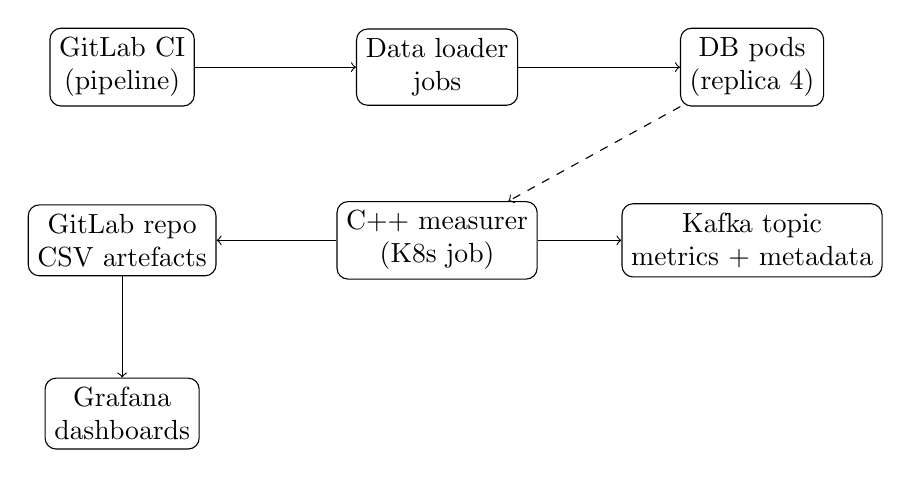
\begin{tikzpicture}[x=1cm,y=1cm]
    \node[draw,rounded corners,align=center] (gitlab) at (0,0) {GitLab CI\\(pipeline)};
    \node[draw,rounded corners,align=center] (loader) at (4,0) {Data loader\\jobs};
    \node[draw,rounded corners,align=center] (db) at (8,0) {DB pods\\(replica 4)};
    \node[draw,rounded corners,align=center] (meas) at (4,-2.2) {C++ measurer\\(K8s job)};
    \node[draw,rounded corners,align=center] (kafka) at (8,-2.2) {Kafka topic\\metrics + metadata};
    \node[draw,rounded corners,align=center] (repo) at (0,-2.2) {GitLab repo\\CSV artefacts};
    \node[draw,rounded corners,align=center] (grafana) at (0,-4.4) {Grafana\\dashboards};

    \draw[->] (gitlab) -- (loader);
    \draw[->] (loader) -- (db);
    \draw[->] (meas) -- (kafka);
    \draw[->] (meas) -- (repo);
    \draw[->] (repo) -- (grafana);
    \draw[->,dashed] (db) -- (meas);
  \end{tikzpicture}
  \caption{Benchmark control and measurement flow. The dashed arrow indicates that the measurer observes the DB via API calls and storage metrics, but does not control the DB logic directly.}
  \label{fig:pipeline}
\end{figure}

\section{Systems Under Test}
\label{sec:sut}

The pipeline includes the following systems. All are deployed with four replicas and placed evenly across the four nodes. Persistent volumes are provisioned via Longhorn.

\begin{itemize}[itemsep=0.25em]
  \item \textbf{PostgreSQL} (relational, MVCC, TOAST) \cite{PostgreSQLToast2026,PostgreSQLVacuum2026}
  \item \textbf{MariaDB/InnoDB} (relational, page-based) \cite{MariaDBCompression2026,MariaDBOptimize2026}
  \item \textbf{ClickHouse} (columnar, MergeTree family) \cite{ClickHouseReplacingMergeTree2026,ClickHouseCompressionCodecs2026}
  \item \textbf{CockroachDB} (distributed SQL, MVCC, LSM/Pebble) \cite{CockroachGCTTL2026,CockroachRowTTL2026}
  \item \textbf{Redis} (in-memory key/value, overwrite semantics) \cite{RedisRDBCompression2026}
  \item \textbf{Apache Kafka} (append-only log, log compaction) \cite{KafkaCompactionDocs2026}
  \item \textbf{MinIO} (S3-compatible object storage; no native content dedup) \cite{MinIOErasureCoding2026,MinIOGitHub2026}
  \item \textbf{ComdareDB} (custom research prototype; planned for a later iteration)
\end{itemize}

\section{Dataset Definition and Duplicate Construction}
\label{sec:dataset}

\paragraph{Duplicate definition.}
A \emph{duplicate} is defined as a \textbf{byte-identical payload} (hash-identical). For JSON payloads, a single canonical serialization is used (stable key order, no whitespace variation) to guarantee byte equality.

\paragraph{Duplicate ratios.}
For each dataset type and size, the workload is generated with duplicate ratios of \textbf{0\%, 50\%, 90\%, 95\%, and 99\%}. This covers both moderate duplication and the extreme regimes in which deduplication-like mechanisms may become visible in physical storage curves.

\paragraph{Placement.}
For each ratio, two placements are executed:
(i) duplicates \emph{within} the same schema/topic/bucket, and
(ii) duplicates \emph{across} distinct schemas/topics/buckets.
This explicitly tests whether any system performs cross-container sharing (rare in general-purpose databases).

\paragraph{Dataset sizes.}
The primary volume targets are \textbf{1\,GB, 5\,GB, and 10\,GB} per run (logical payload volume).

\paragraph{Data types and sources.}
The benchmark mixes synthetic and real-world data to cover typical storage patterns:

\begin{itemize}[itemsep=0.25em]
  \item \textbf{Structured:} time-series tuples, random numeric payloads, and transaction-like rows (SQL-friendly).
  \item \textbf{Semi-structured:} GitHub event logs (JSON) derived from GH Archive. \cite{GHArchive2026}
  \item \textbf{Unstructured:} public-domain text corpora (Project Gutenberg) and media files (images/videos). \cite{ProjectGutenbergTerms2026,NASAMediaGuidelines2026,BlenderOpenMovies2026,KaggleDatasets2026}
\end{itemize}

\section{Workload Stages and DB-Specific Variants}
\label{sec:workload}

Each run consists of staged actions to make the time evolution of storage visible:

\begin{description}[style=nextline, leftmargin=1.5cm, labelwidth=1.3cm, itemsep=0.4em]
  \item[Stage 1] \textbf{Bulk ingest:} one-shot import of a batch (fast path when available, e.g., PostgreSQL \texttt{COPY}).
  \item[Stage 2] \textbf{Incremental ingest:} many small inserts/puts to emulate streaming ingestion and to make compaction/merge effects observable.
  \item[Stage 3] \textbf{Deletion variants:}
    \begin{itemize}[itemsep=0.2em]
      \item \emph{Logical delete} (DELETE / tombstones) without shrink,
      \item \emph{Truncate}-style reset (where supported),
      \item \emph{Drop and recreate} of the dedicated lab schema/topic/bucket (soft reset; PVCs remain).
    \end{itemize}
  \item[Stage 4] \textbf{Refill after delete:} re-ingest to test whether physical space is reclaimed or merely logically freed.
\end{description}

\paragraph{Database-specific switches.}
The literature review indicates that \enquote{deduplication} frequently shows up as a side effect of maintenance. Therefore, a small set of DB-specific variants is tested:

\begin{itemize}[itemsep=0.25em]
  \item \textbf{PostgreSQL:} TOAST compression/storage mode enabled vs. disabled (EXTENDED vs. EXTERNAL where applicable) \cite{PostgreSQLToast2026}; and \texttt{VACUUM} vs. \texttt{VACUUM FULL} for reclamation behavior \cite{PostgreSQLVacuum2026}.
  \item \textbf{ClickHouse:} sequential evaluation of MergeTree-family engines, including (at least) \texttt{MergeTree} (baseline) and \texttt{ReplacingMergeTree} (merge-time dedup). \cite{ClickHouseReplacingMergeTree2026}
  \item \textbf{CockroachDB:} MVCC GC TTL settings (\texttt{gc.ttlseconds}) and row-level TTL jobs as alternative deletion semantics. \cite{CockroachGCTTL2026,CockroachRowTTL2026}
  \item \textbf{Kafka:} baseline delete retention vs. aggressive log compaction (\texttt{cleanup.policy=compact}) as \enquote{deduplication in the broader sense}. \cite{KafkaCompactionDocs2026}
  \item \textbf{MariaDB:} best-practice compression configuration per datatype (page/table compression), compared to a baseline without compression where feasible. \cite{MariaDBCompression2026}
\end{itemize}

Kafka compaction must be configured aggressively (segment sizing and cleaner thresholds) to ensure that compaction happens within experiment time. Relevant topic and broker parameters are taken from the official documentation. \cite{KafkaTopicConfig2026}

\section{Cache Scenarios and Reset Strategy}
\label{sec:cache}

Each run is executed twice:
\textbf{cold-cache} and \textbf{warm-cache}.

\begin{itemize}[itemsep=0.25em]
  \item \textbf{Cold cache:} the DB pod(s) for the system under test are restarted to clear DB-level caches. For ClickHouse, optional explicit cache drop commands (\texttt{SYSTEM DROP ... CACHE}) exist but a pod restart is used for uniformity. \cite{ClickHouseDropCaches2026}
  \item \textbf{Warm cache:} the same run is repeated immediately without restart; this captures the best-case steady-state behavior.
\end{itemize}

OS page cache dropping is not required by the cold-cache definition in this work; however, the infrastructure supports privileged DaemonSets for node-local cache operations if needed.

\section{Metrics and Statistical Treatment}
\label{sec:metrics}

Database research commonly reports throughput and latency distributions, not only means. This benchmark therefore records:

\begin{itemize}[itemsep=0.25em]
  \item \textbf{Throughput:} objects/s and MB/s, both for Stage~1 and Stage~2 (combined and separated).
  \item \textbf{Latency distribution:} mean, max, and percentiles p50/p90/p95/p99 per operation type. \cite{Cooper2010YCSB}
  \item \textbf{Storage footprint:} size-over-time sampled at 100\,ms using Longhorn actual volume size. \cite{LonghornMetrics2026}
\end{itemize}

\paragraph{Effective Data Reduction (EDR).}
To expose replication overhead explicitly, two related ratios are used:

\begin{align}
  \mathrm{EDR}_{\mathrm{cluster}} &= \frac{B_{\mathrm{logical}}}{B_{\mathrm{physical,cluster}}} \label{eq:edr-cluster}\\
  \mathrm{EDR}_{\mathrm{replica}} &= \frac{B_{\mathrm{logical}}}{B_{\mathrm{physical,cluster}} / R} \label{eq:edr-replica}
\end{align}

where $B_{\mathrm{logical}}$ is the logical payload volume inserted once by the client, $B_{\mathrm{physical,cluster}}$ is the total physical footprint across all replicas and storage replicas, and $R$ denotes the effective replication factor (application-level replicas, multiplied by storage-level replicas when applicable). In the current setup, the application-level replica count is 4 and Longhorn is configured with 4 storage replicas, so the effective factor can reach $R=16$ when all layers replicate the same bytes. All overheads (metadata, indices, WAL/logs, compaction artefacts) remain included in $B_{\mathrm{physical,cluster}}$ because they are natural properties of the systems under test. $\mathrm{EDR}_{\mathrm{cluster}}$ therefore answers the question \enquote{How many logical bytes do we get per physical byte in the real cluster?}, while $\mathrm{EDR}_{\mathrm{replica}}$ normalizes out replication to make storage-engine effects comparable.

\paragraph{Repetition and averaging.}
Every point in the run matrix is executed \textbf{three times}. Plots show both the raw trajectories and the averaged curve per configuration; for latency/throughput, mean values and percentile bands are computed across the three repetitions.

\section{Run Matrix and Practical Scope}
\label{sec:run-matrix}

A full-factorial plan is defined by:

\begin{itemize}[itemsep=0.2em]
  \item dataset sizes $\{1,5,10\}$\,GB,
  \item duplicate ratios $\{0,50,90,95,99\}\%$,
  \item placement $\{\text{within},\text{across}\}$,
  \item cache state $\{\text{cold},\text{warm}\}$,
  \item repetitions $=3$,
  \item and DB-specific variants (maintenance/TTL/engine/compaction settings).
\end{itemize}

The base matrix (without DB-specific variants) already yields $3 \cdot 5 \cdot 2 \cdot 2 \cdot 3 = 180$ runs per system. DB-specific variants multiply this number. To keep the project tractable, compression is treated primarily as a \emph{documented capability} in the feature matrix and only as an experimental dimension where it is directly tied to deduplication-like behavior (e.g., PostgreSQL TOAST storage mode, Kafka compaction, ClickHouse merge engines).



\chapter{Conclusion and Outlook}
\label{ch:conclusion}

Deduplication is often presented as a single storage feature, but the literature and the systems survey show that \textbf{redundancy reduction} in real database stacks is distributed across multiple layers: API semantics (upsert/overwrite), engine-level data structures (index layout, MVCC history), background maintenance (vacuum/compaction/merge), and storage subsystems. Classic block-level deduplication (content-addressed chunk sharing) is rare inside general-purpose databases; instead, most systems achieve \emph{deduplication-like} effects indirectly---or not at all.

\section{What deduplication means in this work}

This report uses \emph{physical deduplication} as the guiding notion: whether identical payload bytes lead to shared or eliminated physical representations, and under which conditions this happens. Compression is treated as a related but distinct mechanism: it reduces the footprint of each object instance, while deduplication removes redundant \emph{copies} across objects.

\section{Answering the research questions}

The consolidated literature review and the feature matrix (Appendix~\ref{app:feature-matrix}) make three points explicit:

\begin{enumerate}[itemsep=0.3em]
  \item \textbf{Deduplication is layer-specific.} Mechanisms such as Kafka log compaction or ClickHouse ReplacingMergeTree are \emph{semantic} and operate on keys/rows; they do not imply block-level sharing. Engine-level background work (vacuum, merge, GC) is therefore central to interpreting measured size-over-time curves.
  \item \textbf{Replication dominates physical footprint.} On small clusters with multiple replication layers (DB replicas and storage replicas), the physically consumed bytes may exceed logical payload volume by an order of magnitude. Reporting $\mathrm{EDR}_{\mathrm{cluster}}$ and $\mathrm{EDR}_{\mathrm{replica}}$ side-by-side avoids misleading conclusions.
  \item \textbf{Deletion is not reclamation.} Many databases implement deletion as tombstones or MVCC versioning. Physical space reclamation depends on compaction/vacuum/GC timing and may be delayed or incomplete under the constraint of \enquote{soft resets} (PVCs cannot be destroyed because customer data co-exists on the same systems).
\end{enumerate}

\section{Outlook and open engineering items}

The current benchmark pipeline already supports end-to-end automation and high-frequency size sampling, but several extensions are planned to close remaining gaps:

\begin{itemize}[itemsep=0.25em]
  \item Extend the workload generator from duplication grades (U0/U50/U90) to the full target set (0/50/90/95/99\%).
  \item Implement explicit DB-side maintenance variants (e.g., PostgreSQL \texttt{VACUUM FULL}, ClickHouse \texttt{OPTIMIZE FINAL}) and TTL/GC configurations as first-class pipeline dimensions.
  \item Add systematic cache-reset procedures per DB (where supported) and quantify the impact of pod restarts versus explicit cache-drop commands.
  \item Integrate the custom \textbf{ComdareDB} prototype once it is ready, and compare its physical deduplication behavior to the established systems under identical workloads.
  \item Evaluate CPU affinity pinning (measurer vs. DB pods) as an optional mitigation for measurement overhead on small hardware.
\end{itemize}

Overall, the combination of a consolidated survey and a reproducible experiment framework provides a basis to move from \enquote{deduplication as a buzzword} to \textbf{deduplication as a measurable property} of real database stacks.

\appendix

\chapter{Exhaustive Feature Matrix}
\label{app:feature-matrix}

This appendix provides the detailed feature matrix requested by the supervisor. Each feature is classified as:

\begin{description}[itemsep=0.2em]
  \item[Full] documented and generally available in the system.
  \item[Partial] available only for specific engines/modes, or eventual/limited in scope.
  \item[Indirect] not designed as deduplication, but can reduce redundancy via semantics (overwrite/upsert) or background behavior.
  \item[Missing] not supported.
  \item[N/A] not applicable for this system type.
\end{description}

\begin{center}
\small
\setlength{\tabcolsep}{3pt}
\begin{longtable}{p{4.2cm}p{1.2cm}p{1.2cm}p{1.2cm}p{1.2cm}p{1.2cm}p{1.2cm}p{1.2cm}}
\caption{Deduplication-related feature matrix (core systems).}\label{tab:feature-matrix}\\
\toprule
\textbf{Feature category} &
\textbf{PostgreSQL} &
\textbf{MariaDB} &
\textbf{ClickHouse} &
\textbf{CockroachDB} &
\textbf{Redis} &
\textbf{Kafka} &
\textbf{MinIO} \\
\midrule
\endfirsthead
\toprule
\textbf{Feature category} &
\textbf{PostgreSQL} &
\textbf{MariaDB} &
\textbf{ClickHouse} &
\textbf{CockroachDB} &
\textbf{Redis} &
\textbf{Kafka} &
\textbf{MinIO} \\
\midrule
\endhead
\midrule
\multicolumn{8}{r}{\emph{continued on next page}}\\
\endfoot
\bottomrule
\endlastfoot

\textbf{Storage engine model (high-level)} &
MVCC, heap + B-tree &
InnoDB pages + B-tree &
Columnar parts + merges &
MVCC on LSM (Pebble) &
In-memory structures &
Append-only log segments &
Object storage \\
\addlinespace

\textbf{Insert-time duplicate suppression (idempotency tokens)} &
Indirect (UPSERT/UNIQUE) &
Indirect (UPSERT/UNIQUE) &
Partial (replicated insert dedup) &
Indirect (UPSERT/UNIQUE) &
Indirect (overwrite key) &
Indirect (idempotent producer) &
Indirect (overwrite object key) \\
\addlinespace

\textbf{Row-level/record-level deduplication} &
Indirect (constraints) &
Indirect (constraints) &
Partial (ReplacingMergeTree, merge-time) &
Indirect (constraints) &
Indirect (overwrite) &
N/A &
Missing \\
\addlinespace

\textbf{Key-based compaction (keep last value)} &
N/A &
N/A &
Partial (ReplacingMergeTree semantics) &
N/A &
Indirect (overwrite) &
Full (log compaction) &
Missing \\
\addlinespace

\textbf{Index-level duplicate reduction} &
Full (B-tree dedup) &
Missing &
N/A &
N/A &
N/A &
N/A &
N/A \\
\addlinespace

\textbf{Built-in compression on stored data} &
Full (TOAST) &
Full (InnoDB/page) &
Full (codecs) &
Full (SSTable compression) &
Partial (RDB snapshot) &
Full (record batch) &
Partial (optional; not dedup) \\
\addlinespace

\textbf{Background compaction / merge} &
Partial (VACUUM) &
Partial (purge/OPTIMIZE) &
Full (MergeTree merges) &
Full (LSM compaction) &
N/A &
Full (segment cleaning) &
N/A \\
\addlinespace

\textbf{Explicit \enquote{shrink} operation} &
Partial (VACUUM FULL) &
Partial (OPTIMIZE TABLE) &
Partial (\texttt{OPTIMIZE}) &
Indirect (compaction/GC) &
N/A &
Indirect (segment delete) &
Indirect (delete objects) \\
\addlinespace

\textbf{TTL/retention affecting physical storage} &
Indirect (partition retention) &
Indirect (event scheduler) &
Partial (TTL on tables) &
Full (row TTL + GC TTL) &
N/A &
Full (retention + tombstones) &
Partial (lifecycle) \\
\addlinespace

\textbf{Cross-schema/topic/bucket deduplication} &
Missing &
Missing &
Missing &
Missing &
Missing &
Missing &
Missing \\
\addlinespace

\textbf{Cache reset for cold-cache runs} &
Restart pod &
Restart pod &
Restart pod / SYSTEM DROP CACHE &
Restart node/pod &
Restart pod &
Restart broker/pod &
Restart pod \\
\addlinespace

\end{longtable}
\end{center}

\chapter{DB-Specific Reset, Maintenance, and Measurement Commands}
\label{app:db-commands}

This appendix is intended as a \emph{fill-in} reference: each subsection lists the commands (or API queries) to (i) reset the lab dataset without touching customer data, (ii) trigger maintenance/compaction, (iii) clear caches where possible, and (iv) query internal size statistics (in addition to Longhorn volume size).

\section{PostgreSQL}
\begin{itemize}[itemsep=0.2em]
  \item Reset (soft): \texttt{DROP SCHEMA lab\_user CASCADE; CREATE SCHEMA lab\_user;}
  \item Truncate variant: \texttt{TRUNCATE TABLE ...;}
  \item Maintenance: \texttt{VACUUM (ANALYZE);} vs. \texttt{VACUUM FULL;} \cite{PostgreSQLVacuum2026}
  \item TOAST mode toggle: column storage \texttt{EXTENDED} vs. \texttt{EXTERNAL} \cite{PostgreSQLToast2026}
  \item Internal size queries: \texttt{pg\_database\_size}, \texttt{pg\_total\_relation\_size} (per schema/table)
\end{itemize}

\section{MariaDB / InnoDB}
\begin{itemize}[itemsep=0.2em]
  \item Reset (soft): \texttt{DROP DATABASE lab\_db; CREATE DATABASE lab\_db;} (or drop individual tables if DB-level is not allowed)
  \item Maintenance: \texttt{OPTIMIZE TABLE ...;} \cite{MariaDBOptimize2026}
  \item Compression toggles: InnoDB page/table compression settings (best-practice per datatype). \cite{MariaDBCompression2026}
  \item Internal size queries: \texttt{information\_schema.TABLES} (data\_length/index\_length) per table
\end{itemize}

\section{ClickHouse}
\begin{itemize}[itemsep=0.2em]
  \item Reset (soft): \texttt{DROP TABLE ...;} / \texttt{TRUNCATE TABLE ...;}
  \item Merge/compaction trigger: \texttt{OPTIMIZE TABLE ... FINAL;} (engine dependent)
  \item Dedup engine: \texttt{ReplacingMergeTree} (merge-time row replacement). \cite{ClickHouseReplacingMergeTree2026}
  \item Cache drop (optional): \texttt{SYSTEM DROP MARK CACHE;} and \texttt{SYSTEM DROP UNCOMPRESSED CACHE;} \cite{ClickHouseDropCaches2026}
  \item Internal size queries: \texttt{system.parts}, \texttt{system.tables}, \texttt{system.columns}
\end{itemize}

\section{CockroachDB}
\begin{itemize}[itemsep=0.2em]
  \item Reset (soft): \texttt{DROP TABLE ...;} / \texttt{TRUNCATE ...;} (schema-scoped)
  \item GC TTL: \texttt{gc.ttlseconds} influences MVCC history retention. \cite{CockroachGCTTL2026}
  \item Row-level TTL: configure \texttt{ttl} on tables and observe background TTL jobs. \cite{CockroachRowTTL2026}
  \item Internal size queries: \texttt{SHOW RANGES}, \texttt{crdb\_internal} tables, or admin endpoints (where available)
\end{itemize}

\section{Kafka}
\begin{itemize}[itemsep=0.2em]
  \item Reset (soft): delete and recreate topic, or delete records to a given offset.
  \item Compaction policy: \texttt{cleanup.policy=compact} plus aggressive cleaner parameters. \cite{KafkaCompactionDocs2026,KafkaTopicConfig2026}
  \item Internal size queries: broker log directory size; topic/partition offsets; segment file inspection
\end{itemize}

\section{Redis}
\begin{itemize}[itemsep=0.2em]
  \item Reset (soft): \texttt{FLUSHDB;} (lab DB index) or key-prefix deletion
  \item Persistence compression: RDB snapshot compression option (\texttt{rdbcompression}). \cite{RedisRDBCompression2026}
\end{itemize}

\section{MinIO}
\begin{itemize}[itemsep=0.2em]
  \item Reset (soft): delete objects in lab bucket; keep customer buckets untouched.
  \item No native content deduplication; redundancy is managed via erasure coding/replication. \cite{MinIOErasureCoding2026,MinIOGitHub2026}
\end{itemize}

\chapter{Measurement Appendix Templates}
\label{app:templates}

The following tables are templates to be filled with measured values (or generated from the CSV artefacts). They focus on the core outcome metrics: storage footprint (EDR) and latency/throughput.

\section{EDR overview (cluster-level)}
\begin{table}[h]
\centering
\small
\begin{tabular}{lcccccc}
\toprule
\textbf{System} & \textbf{1GB} & \textbf{5GB} & \textbf{10GB} & \textbf{Dup 0\%} & \textbf{Dup 95\%} & \textbf{Dup 99\%} \\
\midrule
PostgreSQL &  &  &  &  &  &  \\
MariaDB    &  &  &  &  &  &  \\
ClickHouse &  &  &  &  &  &  \\
Cockroach  &  &  &  &  &  &  \\
Redis      &  &  &  &  &  &  \\
Kafka      &  &  &  &  &  &  \\
MinIO      &  &  &  &  &  &  \\
\bottomrule
\end{tabular}
\caption{Template for $\mathrm{EDR}_{\mathrm{cluster}}$ (Eq.~\ref{eq:edr-cluster}). Fill with measured values.}
\end{table}

\section{Latency percentiles (example template)}
\begin{table}[h]
\centering
\small
\begin{tabular}{lcccccc}
\toprule
\textbf{System} & \textbf{p50} & \textbf{p90} & \textbf{p95} & \textbf{p99} & \textbf{max} & \textbf{mean} \\
\midrule
PostgreSQL (insert) &  &  &  &  &  &  \\
MariaDB (insert)    &  &  &  &  &  &  \\
ClickHouse (insert) &  &  &  &  &  &  \\
Cockroach (insert)  &  &  &  &  &  &  \\
Redis (set)         &  &  &  &  &  &  \\
Kafka (produce)     &  &  &  &  &  &  \\
MinIO (put)         &  &  &  &  &  &  \\
\bottomrule
\end{tabular}
\caption{Template for latency distribution reporting (cold-cache, 10\,GB, dup 0\%). Extend by workload stage and duplicate ratios as needed.}
\end{table}

\section{CSV schema}
\begin{verbatim}
timestamp,run_id,system,variant,data_type,data_size_gb,dup_ratio,placement,cache_state,stage,
replica_id,metric,value,unit
\end{verbatim}

\noindent The \texttt{run\_id} encodes all dimensions (system, variant, dataset, cache state, placement, repetition) so that Grafana can group and compare runs reliably.



\end{document}